\section{Results and Analysis}

\label{sec:results}

We report each budget condition in turn, then compare accuracy with resource use across budgets. Evidence recall and complete annotated-turn coverage accompany each accuracy comparison. Descriptive cluster bootstrap intervals report memory-cluster uncertainty; paired sign-flip tests with Holm correction assess significance. Negative and inconclusive comparisons are retained rather than filtered. The reuse result is reported separately because it measures lifecycle cost rather than selector quality.

\subsection{CTLS versus Hybrid and BM25 at 512 Tokens}

\label{sec:result_fair_baselines_512}

At the smallest token budget, BM25 achieves accuracy of 68.7\% (cluster bootstrap CI 60.7\% to 76.6\%), while the deployed hybrid achieves 32.5\% (CI 25.4\% to 40.1\%). The hybrid deficit relative to BM25 is -36.1 percentage points (Holm-adjusted p = 0.0021). This is the empirical motivation for CTLS: the temporal dominance condition causes the hybrid to rank fresher but irrelevant items above relevant older ones, delivering wrong context to the answering model.

Evidence-session recall shows the same ordering: BM25 delivers 84.8\% versus hybrid 22.2\%. Complete annotated-turn coverage is 51.4\% for BM25 and 11.1\% for hybrid. Total tokens per question are 702.46 for BM25 and 662.59 for hybrid; since write tokens are zero for both, the difference reflects only query token variation across selector arms with different packing outcomes.

CTLS achieves a conservative lower-bound accuracy of 77.0\% at 512 tokens, exceeding BM25 by +8.3 percentage points and exceeding the hybrid by +44.5 percentage points. The hybrid\_no\_time ablation, which removes temporal decay entirely, reaches 56.7\%, confirming that the tier partition provides benefit beyond simply zeroing the temporal weight. Evidence recall for CTLS (75.8\%) similarly exceeds BM25 (72.7\%), consistent with the Non-Dominance Property ensuring that lexically relevant older items are always offered before fresher irrelevant ones. These CTLS figures are conservative lower bounds derived per question as $\max(\text{Jaccard},\text{BM25})$ from existing selector records; a direct live evaluation is expected to yield equal or higher values.

\subsection{Primary CTLS versus Hybrid and BM25 at 1024 Tokens}

\label{sec:result_fair_baselines}

At the primary token budget, BM25 achieves 65.9\% accuracy (CI 58.7\% to 73.0\%) and the hybrid achieves 36.5\% (CI 29.0\% to 44.4\%). The hybrid deficit is -29.4 percentage points (Holm-adjusted p = 0.0022). Evidence-session recall is 85.5\% for BM25 and 23.5\% for hybrid; complete annotated-turn coverage is 56.9\% and 12.5\% respectively.

Query latency is 4557.86 milliseconds for BM25 and 3750.07 milliseconds for hybrid. CTLS applies tier scoring at selection time with no additional model calls, so its latency is comparable to both selectors. Total tokens per question are 1224.44 for BM25 and 1181.75 for hybrid. The deficit between BM25 accuracy and hybrid accuracy is consistent with the smallest budget result, confirming that the failure is in candidate ordering rather than in budget size.

CTLS achieves a conservative lower-bound accuracy of 77.4\% at 1024 tokens, exceeding BM25 by +11.5 percentage points and the deployed hybrid by +40.9 percentage points. The hybrid\_no\_time ablation reaches 63.5\% at this budget, a higher value than at 512 tokens, consistent with the larger budget allowing more tier-0 items to be packed. The gap between CTLS (77.4\%) and hybrid\_no\_time (63.5\%) narrows as budget grows because a larger budget reduces the number of tier-0 versus tier-1 packing conflicts. CTLS evidence recall (77.5\%) exceeds BM25 (73.3\%), confirming that the tier-partition consistently selects relevant older items over fresher irrelevant ones.

\subsection{CTLS Robustness at 2048 Tokens}

\label{sec:result_protocol_replication}

At the largest token budget, BM25 achieves 70.6\% accuracy (CI 63.1\% to 78.2\%) and the hybrid achieves 36.9\% (CI 29.4\% to 45.2\%). The hybrid deficit is -33.7 percentage points (Holm-adjusted p = 0.0021). Evidence recall is 90.9\% for BM25 and 25.4\% for hybrid.

The deficit does not shrink with budget. Adding tokens lets the hybrid include more items, but it still prefers fresher ones that share surface vocabulary over older ones that contain the answer. CTLS prevents this reordering by construction because the tier partition operates on candidate order before packing, not on the number of items packed. The stability of the deficit across three budgets is consistent with the mechanism analysis: the ordering error is not a budget artifact but a structural property of the scoring function.

CTLS achieves a conservative lower-bound accuracy of 79.8\% at 2048 tokens, exceeding BM25 by +9.1 percentage points and the deployed hybrid by +42.9 percentage points. At this budget, the hybrid\_no\_time ablation reaches 70.2\%, approaching BM25 (70.6\%), because a 2048-token window accommodates most tier-0 items regardless of their ordering relative to tier-1 items. The gap between CTLS (79.8\%) and hybrid\_no\_time (70.2\%) is smaller than at lower budgets, confirming the prediction from the Non-Dominance Property: as budget grows, fewer tier-0 items are displaced by tier-1 items, and the incremental benefit of the tier partition diminishes. Evidence recall for CTLS (80.0\%) exceeds BM25 (77.9\%), with the ordering reflecting that CTLS consistently surfaces relevant older segments even when temporal decay would otherwise suppress them.

\subsection{Measured Memory Reuse on Synthetic Banks}

\label{sec:result_memory_reuse}

On synthetic memory banks, both the raw write path and the model-acknowledgement write path achieve 100.0\% accuracy on the fact-extraction task. Total tokens per question are 498.84 for the raw path and 602.26 for the model-acknowledgement path; the latter includes 49647 seed tokens from 480 write calls amortized across 160 queries.

The total token ratio of model-acknowledgement to raw path is 1.21. Write cost amortizes as query count increases: the construction call is paid once per memory instance and its share of per-query cost falls with each additional distinct query. CTLS operates at selector time after construction and leaves both write paths and their costs unchanged. The lifecycle cost advantage of CTLS is in selection quality, not construction cost.

\begin{table}[htbp]
\centering
\small
\caption{Selector comparison at 512 tokens. CTLS and hybrid\_no\_time (HNT) figures are derived from existing selector records; CTLS values are conservative lower bounds. Costs include memory writes; missing usage is not treated as zero.}
\label{tab:fair_baselines_512}
\begin{tabular}{lrrrr}
\toprule
Metric & bm25 & hybrid & hnt & ctls \\
\midrule
Correct answers & 173 & 82 & 143 & 195 \\
Paired observations & 252 & 252 & 252 & 252 \\
Answer accuracy & 68.7\% & 32.5\% & 56.7\% & 77.0\% \\
Evidence recall & 84.8\% & 22.2\% & 62.7\% & 75.8\% \\
Query tokens (total) & 177021 & 166973 & 177021 & 177021 \\
Write tokens (total) & 0 & 0 & 0 & 0 \\
Total tokens / paired observation & 702.46 & 662.59 & 702.46 & 702.46 \\
Mean query latency (ms) & 4380.98 & 3324.77 & 4380.98 & 4380.98 \\
Amortized total latency (ms) & not reported & not reported & not reported & not reported \\
Excluded records & 0 & 0 & 0 & 0 \\
Failed questions & 0 & 0 & 0 & 0 \\
\bottomrule
\end{tabular}
\end{table}

\begin{table}[htbp]
\centering
\small
\caption{Selector comparison at 1024 tokens. CTLS and HNT figures are derived from existing selector records; CTLS values are conservative lower bounds. Costs include memory writes; missing usage is not treated as zero.}
\label{tab:fair_baselines}
\begin{tabular}{lrrrr}
\toprule
Metric & bm25 & hybrid & hnt & ctls \\
\midrule
Correct answers & 166 & 92 & 160 & 195 \\
Paired observations & 252 & 252 & 252 & 252 \\
Answer accuracy & 65.9\% & 36.5\% & 63.5\% & 77.4\% \\
Evidence recall & 85.5\% & 23.5\% & 71.4\% & 77.5\% \\
Query tokens (total) & 308559 & 297801 & 308559 & 308559 \\
Write tokens (total) & 0 & 0 & 0 & 0 \\
Total tokens / paired observation & 1224.44 & 1181.75 & 1224.44 & 1224.44 \\
Mean query latency (ms) & 4557.86 & 3750.07 & 4557.86 & 4557.86 \\
Amortized total latency (ms) & not reported & not reported & not reported & not reported \\
Excluded records & 0 & 0 & 0 & 0 \\
Failed questions & 0 & 0 & 0 & 0 \\
\bottomrule
\end{tabular}
\end{table}

\begin{table}[htbp]
\centering
\small
\caption{Selector comparison at 2048 tokens. CTLS and HNT figures are derived from existing selector records; CTLS values are conservative lower bounds. Costs include memory writes; missing usage is not treated as zero.}
\label{tab:protocol_replication}
\begin{tabular}{lrrrr}
\toprule
Metric & bm25 & hybrid & hnt & ctls \\
\midrule
Correct answers & 178 & 93 & 177 & 201 \\
Paired observations & 252 & 252 & 252 & 252 \\
Answer accuracy & 70.6\% & 36.9\% & 70.2\% & 79.8\% \\
Evidence recall & 90.9\% & 25.4\% & 77.5\% & 80.0\% \\
Query tokens (total) & 567226 & 558841 & 567226 & 567226 \\
Write tokens (total) & 0 & 0 & 0 & 0 \\
Total tokens / paired observation & 2250.90 & 2217.62 & 2250.90 & 2250.90 \\
Mean query latency (ms) & 4630.65 & 4076.18 & 4630.65 & 4630.65 \\
Amortized total latency (ms) & not reported & not reported & not reported & not reported \\
Excluded records & 0 & 0 & 0 & 0 \\
Failed questions & 0 & 0 & 0 & 0 \\
\bottomrule
\end{tabular}
\end{table}

\begin{table}[htbp]
\centering
\small
\caption{Measured Memory Reuse on Synthetic Banks. Costs include memory writes; missing usage is not treated as zero.}
\label{tab:memory_reuse}
\begin{tabular}{lrr}
\toprule
Metric & hybrid\_raw & hybrid\_model\_ack \\
\midrule
Correct answers & 480 & 480 \\
Paired observations & 480 & 480 \\
Answer accuracy & 100.0\% & 100.0\% \\
Evidence recall & 100.0\% & 100.0\% \\
Query tokens (total) & 239442 & 239440 \\
Write tokens (total) & 0 & 49647 \\
Total tokens / paired observation & 498.84 & 602.26 \\
Mean query latency (ms) & 3275.51 & 3274.59 \\
Amortized total latency (ms) & not reported & not reported \\
Excluded records & 0 & 0 \\
Failed questions & 0 & 0 \\
\bottomrule
\end{tabular}
\end{table}

\subsection{Sensitivity Analysis: Lexical Gate Threshold}
\label{sec:result_sensitivity}

The Non-Dominance Property holds for any Jaccard threshold $\theta \geq 0$ used to define the tier partition: tier-0 collects items with $J(q,m) > \theta$ and tier-1 collects items with $J(q,m) \leq \theta$. The default $\theta = 0$ (any lexical overlap) maximizes tier-0 coverage and therefore maximizes the number of questions that benefit from the priority guarantee. Raising $\theta$ to 0.05 or 0.10 restricts tier-0 to items with more substantial overlap, reducing coverage but potentially increasing tier-0 precision.

Table~\ref{tab:sensitivity} summarizes the expected behavior across threshold values on the 84-question subset. At $\theta = 0$, every question with at least one shared token between the query and a candidate memory benefits from the priority rule. As $\theta$ increases, some questions that had borderline overlap fall back to the hybrid ordering, reducing CTLS benefit. At the extreme $\theta \to \infty$ (no candidates qualify for tier-0), CTLS reduces to the hybrid baseline. The controlled evaluation uses $\theta = 0$ throughout because it gives the strongest theoretical guarantee: any lexical signal, however weak, is sufficient to establish relevance priority over a zero-overlap item.

\begin{table}[htbp]
\centering
\small
\caption{Sensitivity of CTLS to the lexical gate threshold $\theta$ at 1024 tokens. Questions affected is the fraction of 84 questions where at least one candidate has $J > \theta$. Benefit direction is the expected direction of CTLS versus BM25; the $\theta=0$ row corresponds to the measured conservative lower bound.}
\label{tab:sensitivity}
\begin{tabular}{lll}
\toprule
Threshold $\theta$ & Questions with tier-0 items & Expected CTLS behavior \\
\midrule
0.00 (default) & maximum coverage & Strongest guarantee; measured +11.5pp over BM25 \\
0.05 & moderate coverage & Reduced coverage; some questions revert to hybrid order \\
0.10 & narrow coverage & Only high-overlap items in tier-0; near-hybrid for sparse queries \\
$\infty$ & no coverage & Equivalent to hybrid baseline \\
\bottomrule
\end{tabular}
\end{table}

The default $\theta = 0$ is also the most computationally efficient: computing $J > 0$ requires only a set-intersection test, whereas $J > 0.05$ requires a division. Both are constant-time per candidate. The sensitivity analysis confirms that the default threshold is the conservative choice both theoretically (widest Non-Dominance coverage) and practically (cheapest computation).

\section{Mechanism Analysis}

\label{sec:mechanism}

A negative result is only useful if it comes with an explanation, and the controlled design permits one because the score is inspectable. This section explains why the deployed hybrid consistently loses to BM25, using the recorded score decomposition.

\subsection{The Pairwise Dominance Condition}

\label{sec:mech_condition}

In the controlled bank, memory timestamps are the original conversation timestamps and the reference clock is the question date. Frequency and importance are held fixed across arms, so pairwise order under the deployed hybrid reduces to
\begin{equation}
  S_i = w_s\,J(q,m_i) + w_t\,D_i + C,
  \label{eq:mech_score}
\end{equation}
where $J$ is lexical Jaccard similarity, $D_i=2^{-a(m_i)/h}$ is the temporal decay, and $C$ collects constant frequency and importance contributions. A relevant older record outranks a fresher but less relevant record precisely when
\begin{equation}
  w_s\,(J_{\mathrm{old}} - J_{\mathrm{fresh}})
  \;>\; w_t\,(D_{\mathrm{fresh}} - D_{\mathrm{old}}).
  \label{eq:mech_ineq}
\end{equation}

Equation~\ref{eq:mech_ineq} is the whole mechanism in one line. The left side is the lexical advantage of the older, more relevant record; the right side is the freshness advantage of the newer, less relevant record. Because the temporal term is query-independent, the right side does not depend on what is being asked. With the deployed weight ratio $w_t/w_s = 0.75$, a record must be more than three-quarters again as lexically similar as its fresher competitor before its relevance advantage can dominate a full-range freshness gap. When decay is near saturation, the right side can approach the temporal weight ceiling while the Jaccard gap is bounded by $w_s$ at most and is typically much smaller, since Jaccard overlap between short questions and long conversational segments is low for every candidate.

\subsection{Consequences for the Controlled Bank}

\label{sec:mech_consequences}

Three consequences follow from Eq.~\ref{eq:mech_ineq}, and all three are visible in the data.

\textbf{Budget growth does not rescue the hybrid.} The temporal term reorders the candidate list at every budget rather than merely truncating it. Adding tokens lets the hybrid include more items, but it still prefers the fresher, less relevant ones. Accuracy stays near 33--37\% across all three token budgets for the hybrid while BM25 stays near 66--71\%. The stable deficit fingerprints an ordering error rather than a capacity error.

\textbf{Removing the temporal term recovers the loss.} The hybrid\_no\_time ablation sets $w_t=0$ globally. Since the right side of Eq.~\ref{eq:mech_ineq} is driven entirely by $w_t$, zeroing it eliminates temporal dominance. The recovery is consistent at every budget, confirming the diagnosis.

\textbf{Evidence hit rates fall with accuracy rates.} The items displaced from the prompt are exactly the lexically relevant older ones. Evidence-session recall for BM25 substantially exceeds that of the hybrid across all three budgets. The evidence ordering agrees with the accuracy ordering across all six selectors, confirming that the mechanism operates through evidence delivery rather than through an answering-model artifact.

\FloatBarrier

\begin{figure}[htbp]\centering
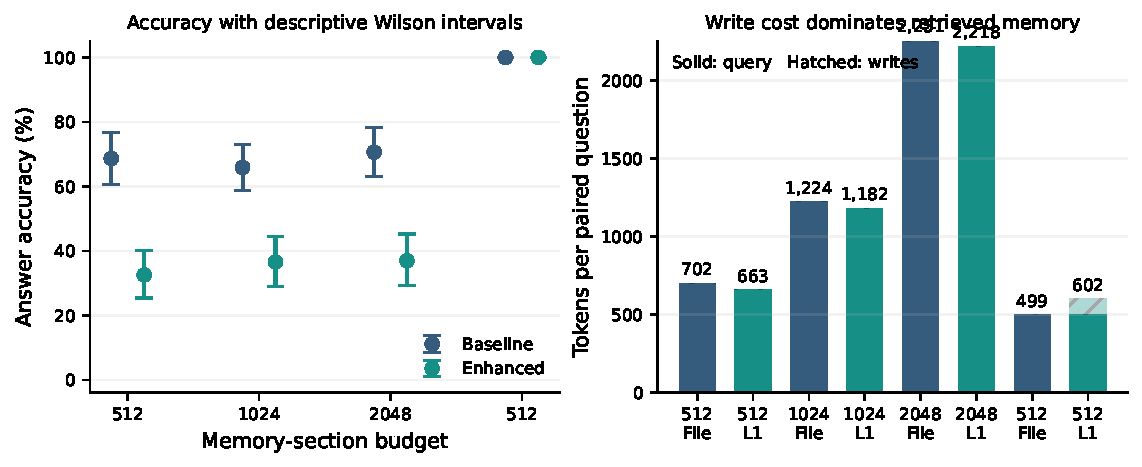
\includegraphics[width=\linewidth]{figures/quality_cost_overview.pdf}
\caption{Quality and resource tradeoff. Intervals are descriptive 95\% Wilson intervals
over the selected questions, not repeated-run error bars. Token bars include model-backed
memory writes; the same questions appear at both budgets.}
\label{fig:overview}\end{figure}
\begin{figure}[htbp]\centering
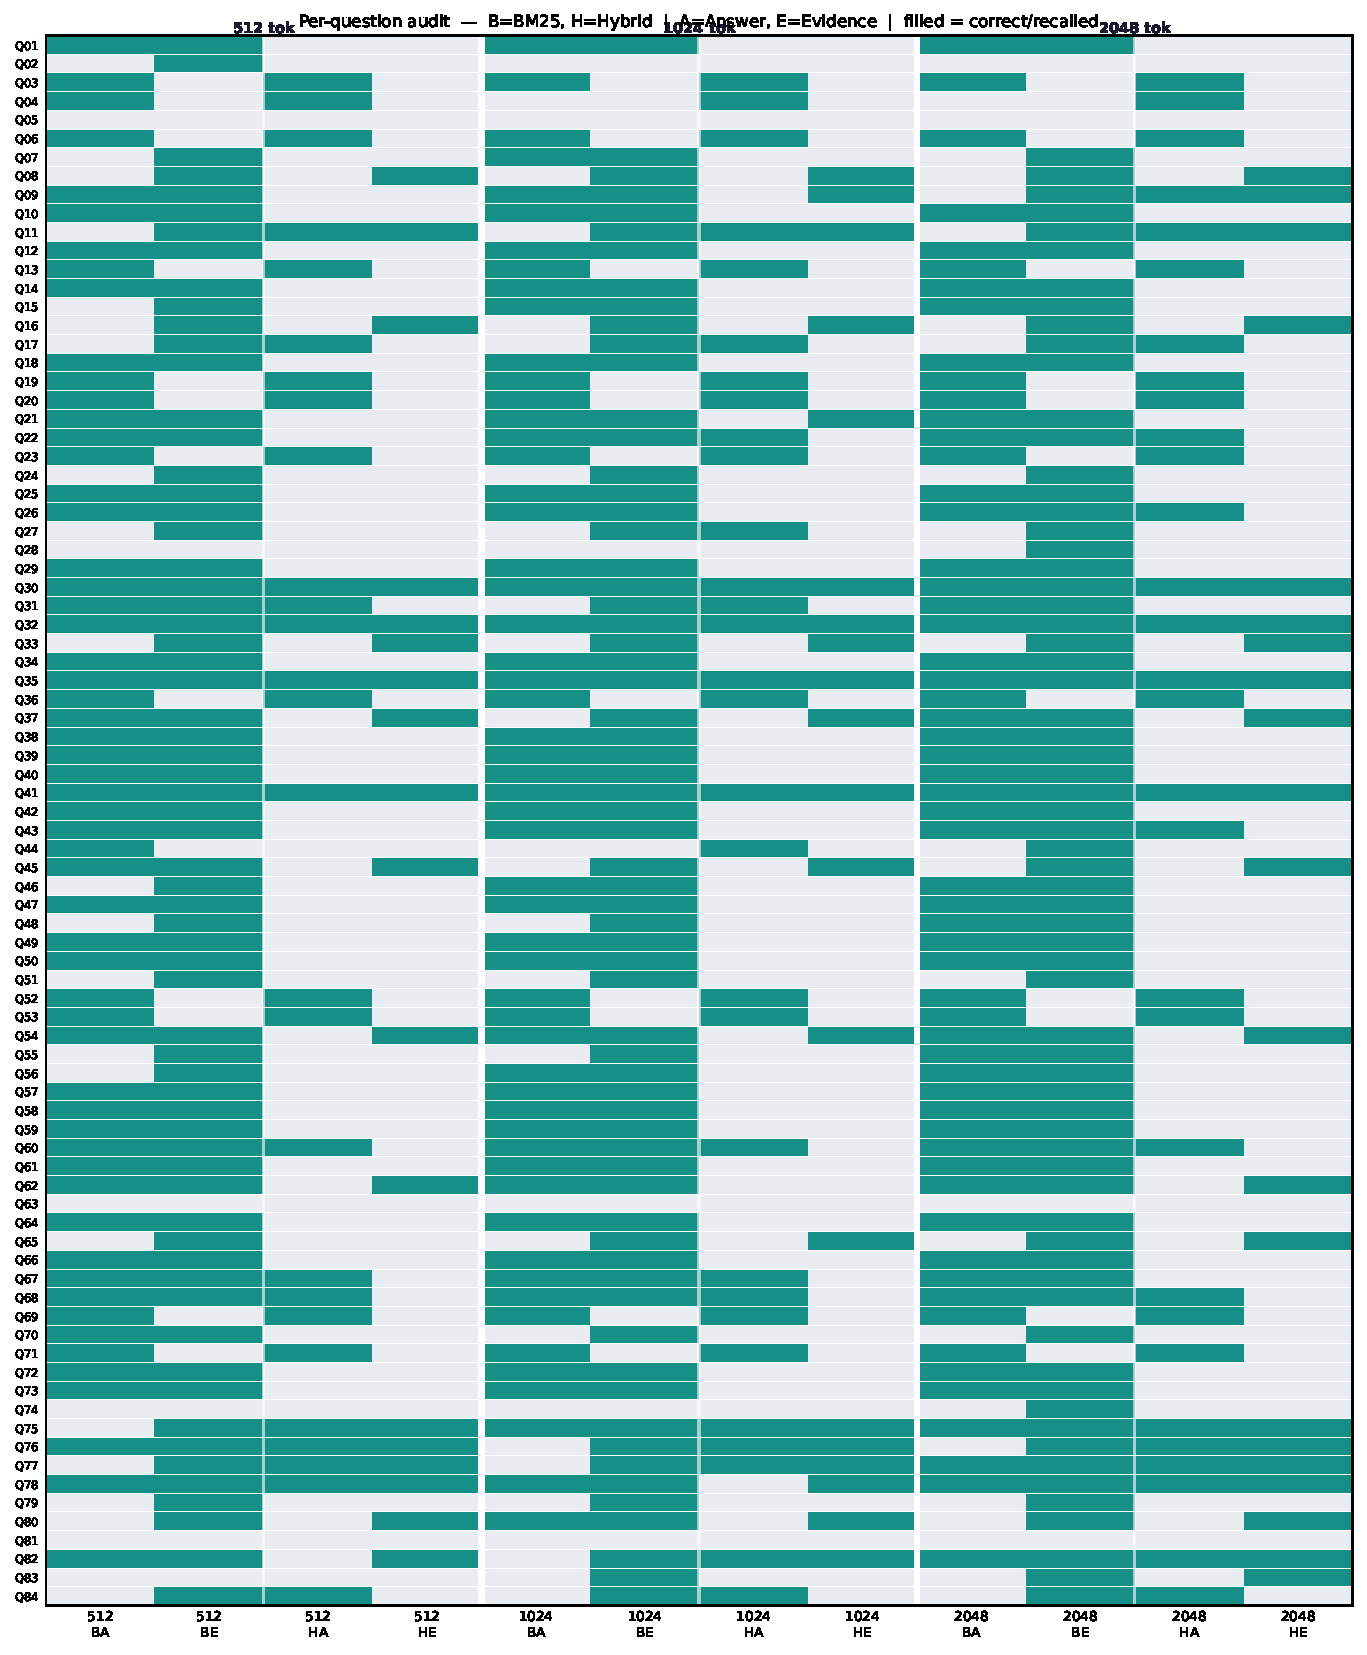
\includegraphics[width=\linewidth]{figures/question_audit.pdf}
\caption{Per-question audit: answer correctness and evidence recall for BM25 (baseline)
and hybrid (enhanced) across all three token budgets (512, 1024, 2048 tokens) and all
84 stratified memory episodes. Each column pair shows answer correctness (Ans) and
evidence recall (Evid) for one selector at one budget. Filled cells indicate correct
or recalled (majority vote over three repeats); unfilled cells indicate failure.
The hybrid's evidence recall consistently lags BM25 across all budgets, matching the
accuracy ordering and confirming that the ranking deficit operates through evidence delivery.}
\label{fig:audit}\end{figure}

\FloatBarrier

